\section{Columbia Game Corpus}

\begin{figure}[t]
\centering
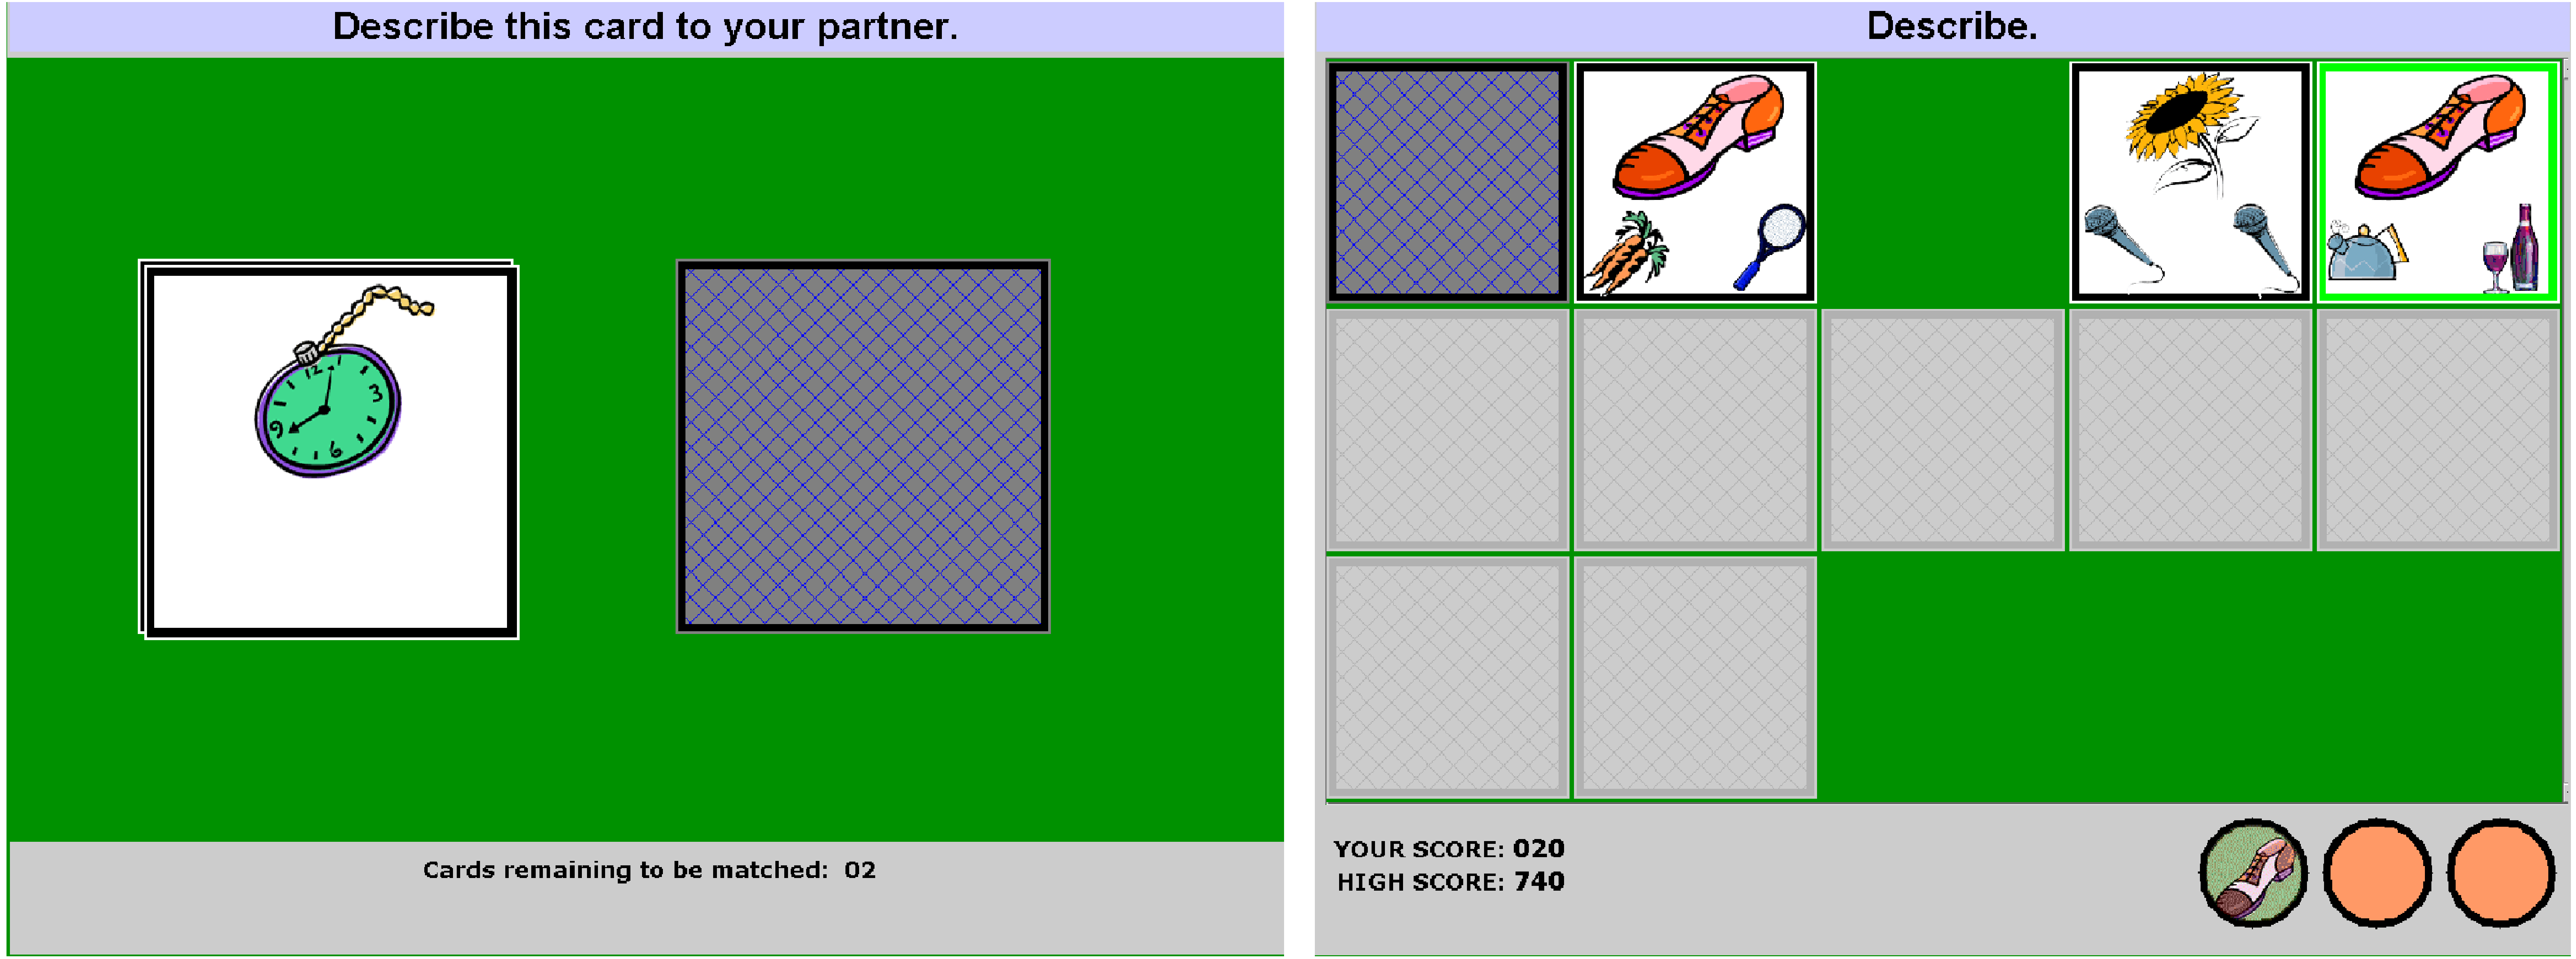
\includegraphics[width=10cm]{images/columbia_games_card_game.png}
\caption{Juego del Columbia Games - Juego de Cartas}
\end{figure}


\newcommand{\cardgame} {\emph{Juego de cartas}}
\newcommand{\objectgame} {\emph{Juego de objetos}}


Nuestro corpus \cite{GRAV2009} consiste en doce conversaciones diádicas (i.e., con dos participantes) entre trece personas angloparlantes distintas. Todos los participantes reportaron hablar Inglés Americano Estándar, y no tener problemas de audición. La edad de los participantes se encuentra en el rango de los 20 a 50 años.

Las grabaciones se hicieron en 44 kHz, 16 bits con un canal separado para cada hablante; luego fueron guardadas en 16 kHz para el presente estudio. Cada sesión duró aproximadamente 45 minutos, totalizando 9 horas de
diálogos, 70.259 palabras (2.037 únicas) para todo el cuerpo de datos.

En cada sesión, se sentó a dos participantes (quienes no se conocían previamente) en una cabina profesional de grabación, cara a cara a ambos lados de una mesa, y con una cortina opaca colgando entre ellos para evitar la comunicación visual. Los participantes contaron con sendas computadoras portátiles conectadas entre sí, en las cuales jugaron una serie de juegos simples que requerían de comunicación verbal. El primero de ellos, un juego de cartas que consta de tres instancias que no consideramos en el presente estudio. Luego de ésto, pasaron al juego que analizamos.

\subsection{Juego de Objetos}

Luego de completar el juego de cartas, los sujetos siguieron interactuando a través del juego de objetos. En éste, la pantalla de cada jugador mostró un tablero con varios objetos, entre 5 y 7, como se ve en la figura \ref{objects_game}. Todos ellos se encuentran cercanos, con excepción de uno, a quien llamamos el Objetivo.

Para uno de los jugadores (el Descriptor) el Objetivo apareció en una posición aleatoria entre otros objetos. Para el otro jugador, a quien llamaremos el Seguidor, el Objetivo apareció en la parte baja de la pantalla. Entonces, al Descriptor se le encargó describir la posición del Objetivo de manera que el Seguidor pudiera mover su representación del objeto a la misma posición en su pantalla. Luego de una negociación entre ambos jugadores para decidir la mejor posición del objeto, se les asignó a los jugadores una puntuación entre 1 y 100 puntos de acuerdo a qué tan acertado fue el posicionamiento del Seguidor.

\begin{figure}[]
\centering
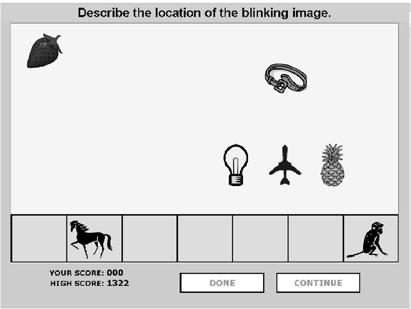
\includegraphics[width=10cm]{images/columbia_games.jpg}
\caption{Juego de objetos del Columbia Games}
\label{objects_game}
\end{figure}


Este juego tomó lugar durante 14 tareas. En las primeras cuatro, uno de los sujetos tomó el papel del Descriptor; en los siguientes cuatro invirtieron roles, y en los finales seis fueron alternando.

\subsection{Anotaciones sobre comportamiento social}

Varios aspectos del comportamiento de los jugadores durante los juegos de objetos fueron anotados mediante la herramienta de crowdsourcing \emph{Mechanical Turk}. Cada anotador escuchó un clip de un juego y tuvo que responder a las siguientes preguntas (para cada uno de los sujetos):

\begin{itemize}
  \item ¿el sujeto parece comprometido con el juego?
  \item ¿el sujeto dirige la conversación?
  \item ¿el sujeto contribuye para el éxito del equipo?
  \item ¿el sujeto alienta a su compañero?
  \item ¿el sujeto se expresa correctamente?
  \item ¿al sujeto no le agrada su compañero?
  \item ¿el sujeto le hace difícil hablar a su compañero?
  \item ¿el sujeto intenta acaparar la conversación?
\end{itemize}

entre otras. Cada uno de estos clips fue puntuado por cinco anotadores, que respondieron por sí o por no. El puntaje que recibe cada una de las preguntas (a las cuales llamaremos a partir de ahora \emph{variables sociales}) consiste en la cantidad de respuestas afirmativas que recibió, teniendo un rango de 0 a 5.

\subsection{Extracción de variables acústico/prosódicas}

El set de herramientas \emph{Praat} fue utilizado para extraer automáticamente las variables acústico/prosódicas del corpus, para cada tarea de éste. Las variables que medimos fueron el tono, la intensidad, la proporción de vocalizaciones, jitter, shimmer, cantidad de sílabas, cantidad de fonemas, y la proporción de ruido sobre armónicos. Éstos atributos fueron medidos en cada uno de los segmentos de habla del corpus.

Repasemos algunos conceptos que necesitamos para definir las variables acústicas.

\begin{itemize}
  \item \emph{f0} refiere a la frecuencia fundamental de una onda, que es el recíproco del período de ésta. El \emph{tono} o \emph{pitch} es la percepción que tenemos de la frecuencia fundamental, que nos marca cuán agudos o graves son los sonidos.
  \item \emph{ENG} refiere al volumen o intensidad de la onda. Ésta se mide por la amplitud de la onda, y es la percepción de cuán fuerte es el sonido.
  \item \emph{jitter} se refiere a los desplazamientos de la onda de la verdadera periodicidad.
  \item \emph{shimmer} se refiere, de manera similar al jitter, a la variación de la onda pero respecto de la amplitud
  \item Un \emph{fonema} es la articulación mínima de un sonido, tanto de vocales como de consonantes. Ejemplos de fonemas son los sonidos de las letras u, a, s, k en español.
  \item El \emph{noise-to-harmonics} ratio puede considerarse como una medida de calidad de la voz, que cuantifica la proporción de ruido que hay en ésta.
\end{itemize}


En la siguiente tabla describimos más detalladamente cada una de ellas. Recordemos nuevamente que estas features son medidas en un intervalo.

\begin{figure}[h!]
\centering
\resizebox{\textwidth}{!}{
\begin{tabular} {|c|c|}
  \hline
  Variable a/p & Descripción \\
  \hline
  \hline
  \FOMEAN & Valor medio de la frecuencia fundamental \\\hline
  \FOMAX  & Valor máximo de la frecuencia fundamental \\\hline
  \ENGMEAN & Valor medio de la intensidad \\\hline
  \ENGMAX & Valor máximo de la intensidad \\\hline
  \TOTFRAMES & Proporción de frames vocalizados sobre totales \\\hline
  \NOISETOHARMONICS & Noise-to-harmonics descripto anteriormente \\\hline
  \LOCALSHIMMER & Shimmer medido \\\hline
  \SYLCOUNT & Cantidad de sílabas \\\hline
  \SYLAVG & Cantidad de sílabas sobre la longitud del intervalo \\\hline
  \PHONCOUNT & Cantidad de fonemas \\\hline
  \PHONAVG & Cantidad de fonemas sobre la longitud del intervalo \\\hline
\end{tabular}
}
\end{figure}

\nota{En los lugares donde digo frame, ¿puedo decir fonemas? No explico bien a qué me refiero con frame}
\nota{Cuál es la relación entre NHR y VCD2TOTFRAMES? Uno es 1 -<el otro>?}
\nota{Agustín, pasame más tela para cortar de jitter, shimmer y NHR}



